\chapter{Estudo de Caso: Rede Wi-Fi no Bloco Didático do IFCE campus Tauá}
\label{cap:cap:estudo-de-caso}

\section{IFCE campus Tauá}
\label{sec:ifce-taua}

O Instituto Federal de Educação, Ciência e Tecnologia do Ceará conta com 32 campi em funcionamento distribuídos por todo o estado. O \textit{campus} de Tauá do IFCE, foi inaugurado em 20 de novembro de 2009. O \textit{campus} abrange principalmente os municípios de Aiuaba, Arneiroz, Quiterianópolis e Parambu, e recebe alunos de várias outras regiões por meio do Sistema de Seleção Unificada (SISU) do Ministério da Educação (MEC) \cite{ifceTaua2019}.

O \textit{campus} Tauá oferta atualmente os cursos técnicos integrados em Redes de Computadores e Agropecuária e os cursos superiores de Tecnologia de Telemática e Licenciatura em Letras com habilitação em Inglês e Português. No semestre letivo 2019.1, o \textit{campus} conta com mais de 400 alunos matriculados \cite{ifceTaua2019}.

A estrutura física do IFCE Tauá pode ser dividida em duas partes principais: a primeira conta com a instalação original do projeto (inaugurada em 2009), onde está inserida a administração, os laboratórios e a biblioteca; a segunda representa o Bloco Didático, inaugurado em 5 de julho de 2016, o qual abriga nove salas de aula, a coordenadoria de cursos e os laboratórios de informática e eletromagnetismo. O presente trabalho desenvolvido-se no Bloco Didático da instituição, já que este concentra as salas de aula, o que resulta em um grande fluxo de alunos pela área.

O \textit{campus} Tauá conta com diversas atividades de pesquisa, extensão e ensino exercidas por discentes, docentes e técnicos. Assim, a instituição, visando atender a comunidade acadêmica, disponibiliza uma infraestrutura de rede sem fio no \textit{campus}.

Na \autoref{fig:vista-campus} tem-se uma visão total da área do \textit{campus}, delimitada pela marcação em vermelho, que é composto pelo bloco inicial do projeto de 2009, destacado em azul, pelo Bloco Didático, em verde, e, por fim, pela quadra poliesportiva localizada mais ao topo da imagem.

\begin{figure}[H]
	\centering
	\Caption{\label{fig:vista-campus}Visão aérea do IFCE \textit{campus} Tauá.}	
	\UECEfig{}{
		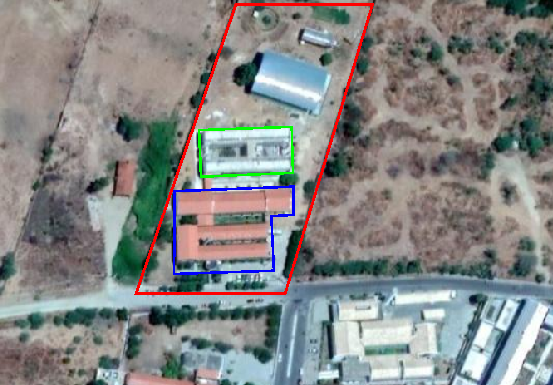
\includegraphics[scale=1]{figuras/ifce-taua-maps.pdf}
	}{
		\Fonte{\citeonline{GoogleMaps}.}
	}	
\end{figure}

\section{Infraestrutura da rede \textit{wireless}}
\label{sec:infraestrutura-wireless}

A instituição conta com uma infraestrutura de rede sem fio com vários pontos de acesso distribuídos em diversos locais de sua área. No bloco 1 (bloco inicial) encontram-se a maior concentração de pontos de acesso, destinados a suprir as necessidades administrativas e de pesquisas desenvolvidas no \textit{campus}. Para o segundo andar Bloco Didático, há a presença de dois pontos de acesso: um destinado aos estudantes e o outro aos professores, ambos localizados na sala de coordenação e indicados pelos marcadores conforme ilustra a \autoref{fig:local-ap}. Para o primeiro andar, não existe ponto de acesso instalados. Entretanto, todos os pontos de acesso no \textit{campus} são protegidos com senhas de acesso alfanuméricos distintas.

\begin{figure}[H]
	\centering
	\Caption{\label{fig:local-ap}Localização dos pontos de acesso no 2º andar do Bloco Didático.}	
	\UECEfig{}{
		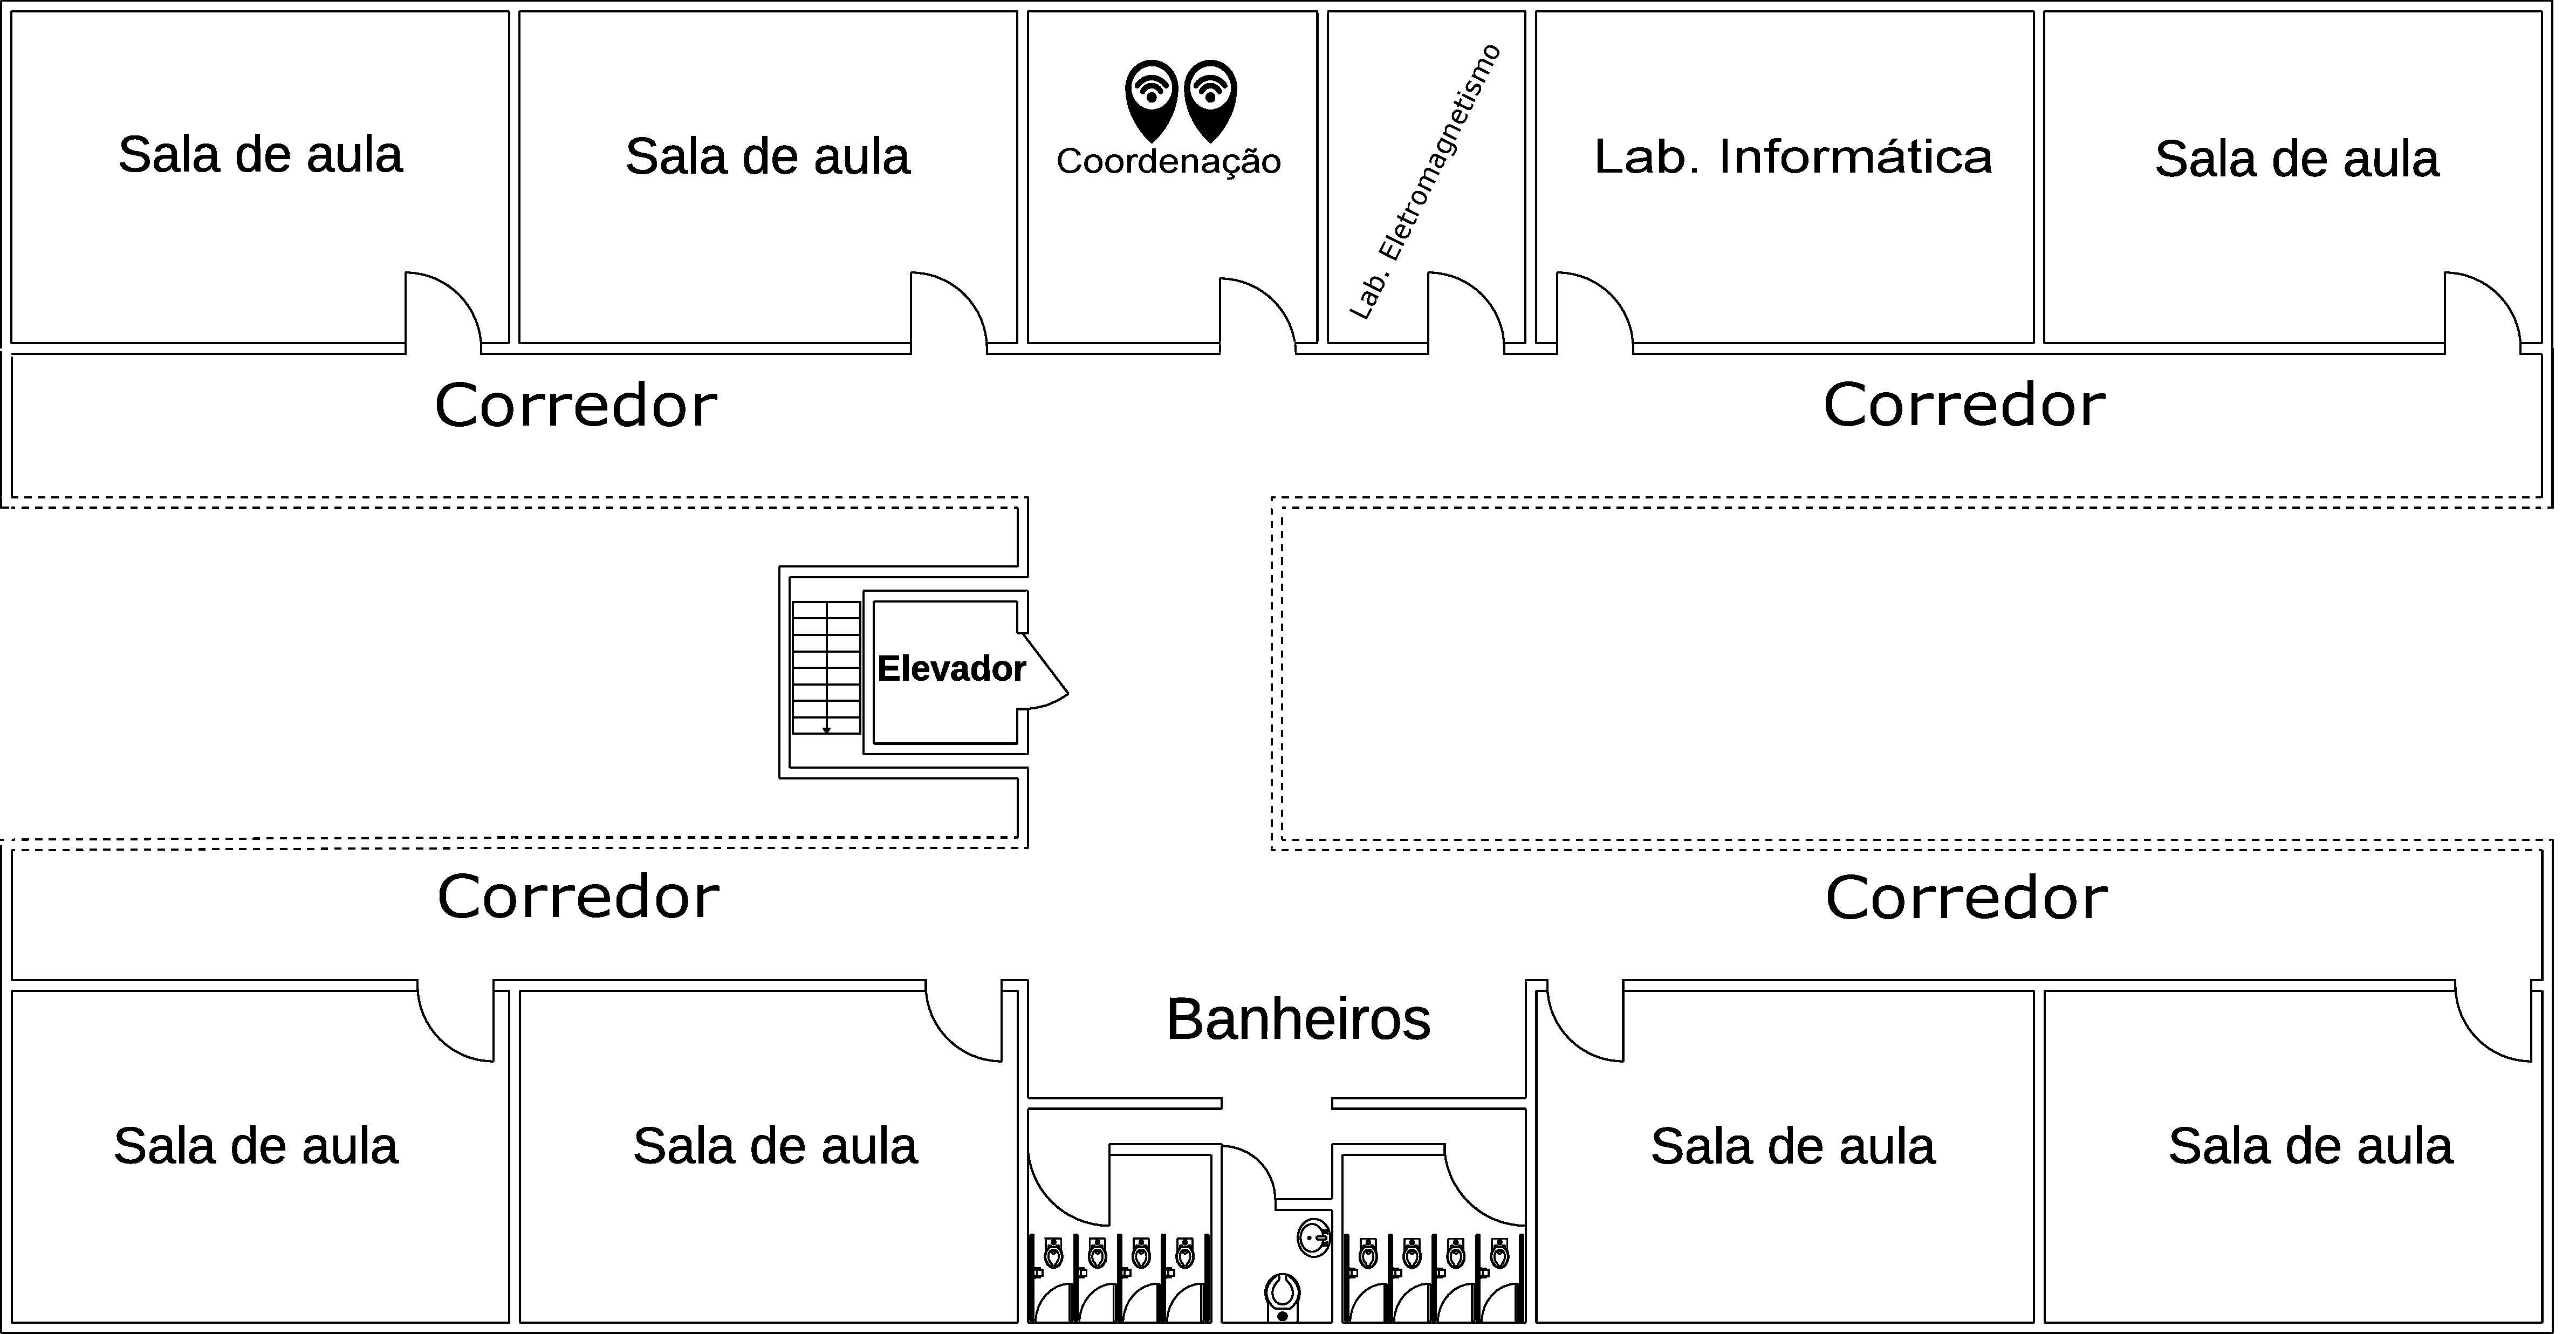
\includegraphics[scale=.18]{figuras/APs_Bloco_Andar_2_01.pdf}
	}{
		\Fonte{Autor.}
	}	
\end{figure}

A Internet disponibilizada no IFCE Tauá é acessível tanto para aqueles que estudam na instituição ou trabalham, como também para visitantes, desde que tenham a senha de acesso. A rede sem fio é dividida de forma a atender cada setor que compõe a organização institucional do \textit{campus}. Isso quer dizer que para os frequentadores da biblioteca existe uma rede específica para eles; para os professores da mesma forma. No entanto, não há restrições para que cada categoria de usuários utilize sua rede própria, cada usuário é livre para associar-se a qualquer ponto de acesso disponível.

As configurações que podem ser encontradas nos pontos de acesso variam de equipamentos que operam na frequência de 2,4 GHz chegando até ao modo \textit{dual band}.

\section{Softwares utilizados}
\label{sec:softwares-utiliados}

Para que sejam realizados os testes iniciais de \textit{site survey} numa rede sem fio é necessário a utilização de \textit{software(s)} dedicado(s) que permita(m) capturar as informações necessárias que possibilitarão avaliar o funcionamento da rede. Neste trabalho foram utilizados dois \textit{softwares}: um para a visualização das redes disponíveis no local alvo (Xirrus Wi-Fi Inspector) e o outro para a geração dos mapas de intensidade de sinal (Ekahau HeatMapper).

Como descrito na capítulo 3, com Xirrus Wi-Fi Inspector, é fácil encontrar redes \textit{wireless} disponíveis, sendo totalmente gratuito. Além disso, a página principal dele exibe quatros campos diferentes que podem ser expandidos para uma visualização mais detalhada: \textit{Radar}, \textit{History}, \textit{Connection} e \textit{Networks}. Cada um possui algumas funções específicas, mas para a proposta deste trabalho, apenas o campo \textit{Networks} foi explorado, já esta janela exibe as informações detalhadas das redes detectadas em determinada área (\autoref{fig:software-xirrus}).

\begin{figure}[H]
	\centering
	\Caption{\label{fig:software-xirrus}Tela de \textit{Networks} do Xirrus Wi-Fi Inspector.}	
	\UECEfig{}{
		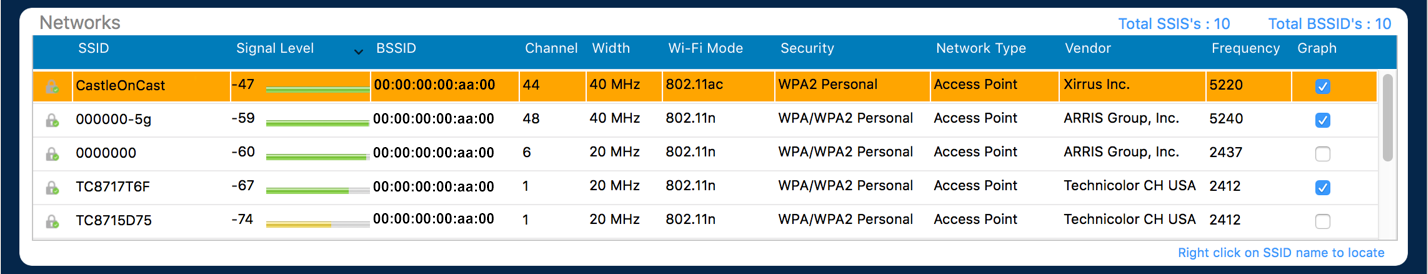
\includegraphics[scale=.41]{figuras/inspector_layout_Riverbed_Networks.png}
	}{
		\Fonte{Autor.}
	}	
\end{figure}

Na janela \textit{Networks} são apresentadas algumas informações dos pontos de acessos descobertos, descritas a seguir:

\begin{compactitem}
	\item \textbf{SSID}: representa o nome da rede sem fio, usado para identificar a mesma, é necessário para associar-se ao ponto de acesso.
	\item \textbf{\textit{Signal Level}:} apresenta a potência do sinal recebido do ponto de acesso em dBm.
	\item \textbf{\textit{Wi-Fi Mode}:} apresenta a versão do padrão 802.11 configurado no ponto de acesso.
	\item \textbf{\textit{Security}:} exibe o protocolo de segurança utilizado pela rede sem fio.
	\item \textbf{\textit{Vendor}:} mostra qual o nome do fabricante do equipamento.
	\item \textbf{BSSID, do inglês, \textit{Basic Service Set Identifier}}: mostra o endereço físico do dispositivo da rede Wi-Fi, que no caso é o endereço MAC (do inglês, \textit{Media Access Control}).
	\item \textbf{\textit{Channel}:} exibe o canal de frequência que o ponto de acesso está utilizando.
	\item \textbf{\textit{Frequency}:} representa a frequência utilizada por um determinado ponto de acesso, podendo ser 2.4 GHz ou 5 GHz.
	\item \textbf{\textit{Network Type}:} exibe o tipo de operação do dispositivo que opera a rede Wi-Fi, seja ponto de acesso ou \textit{ad hoc}.
	\item \textbf{\textit{Graph}:} caixa de seleção para ativar/desativar a representação gráfica do nível de sinal da rede Wi-Fi ao longo do tempo.
\end{compactitem}
	
Já para a criação de mapas de calor dos sinais de radiofrequência, o programa utilizado foi o Ekahau HeatMapper, também descrito no capítulo anterior. Com ele é possível descobrir a cobertura de uma rede Wi-Fi padrão 802.11n/b/g a partir da visualização do mapa de calor obtido na coleta de dados em diversos pontos espalhados pelo local.

O programa possibilita ao usuário escolher um arquivo de seu computador que representa a planta baixa do ambiente de interesse, para assim marcar os pontos onde as medidas de potência foram capturadas e posteriormente a coloração. Esse processo é representado pela \autoref{fig:software-ekahau}.

\begin{figure}[H]
	\centering
	\Caption{\label{fig:software-ekahau}Geração do mapa de calor no Ekahau HeatMapper.}	
	\UECEfig{}{
		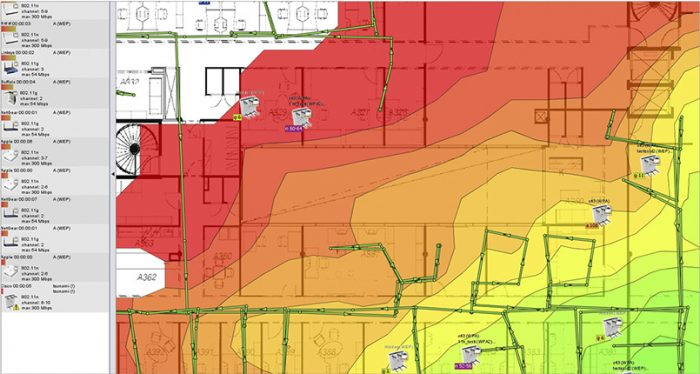
\includegraphics[scale=.5]{figuras/heatmapper-700x374.jpg}
	}{
		\Fonte{\cite{Ekahau2019}.}
	}	
\end{figure}

\section{Equipamento utilizado}
\label{equipamento-utilizado}

Para poder dar início nas medições dos níveis de potência foi utilizado um \textit{notebook} Positivo S14BW01 (\autoref{fig:notebook}) com os \textit{softwares} Xirrus Wi-Fi Inspector e Ekahau HeatMapper instalados e configurados. As especificações do computador podem ser visualizadas na \autoref{tab:carac-notebook}.

\begin{figure}[H]
	\centering
	\Caption{\label{fig:notebook}Notebook Positivo S14BW01.}	
	\UECEfig{}{
		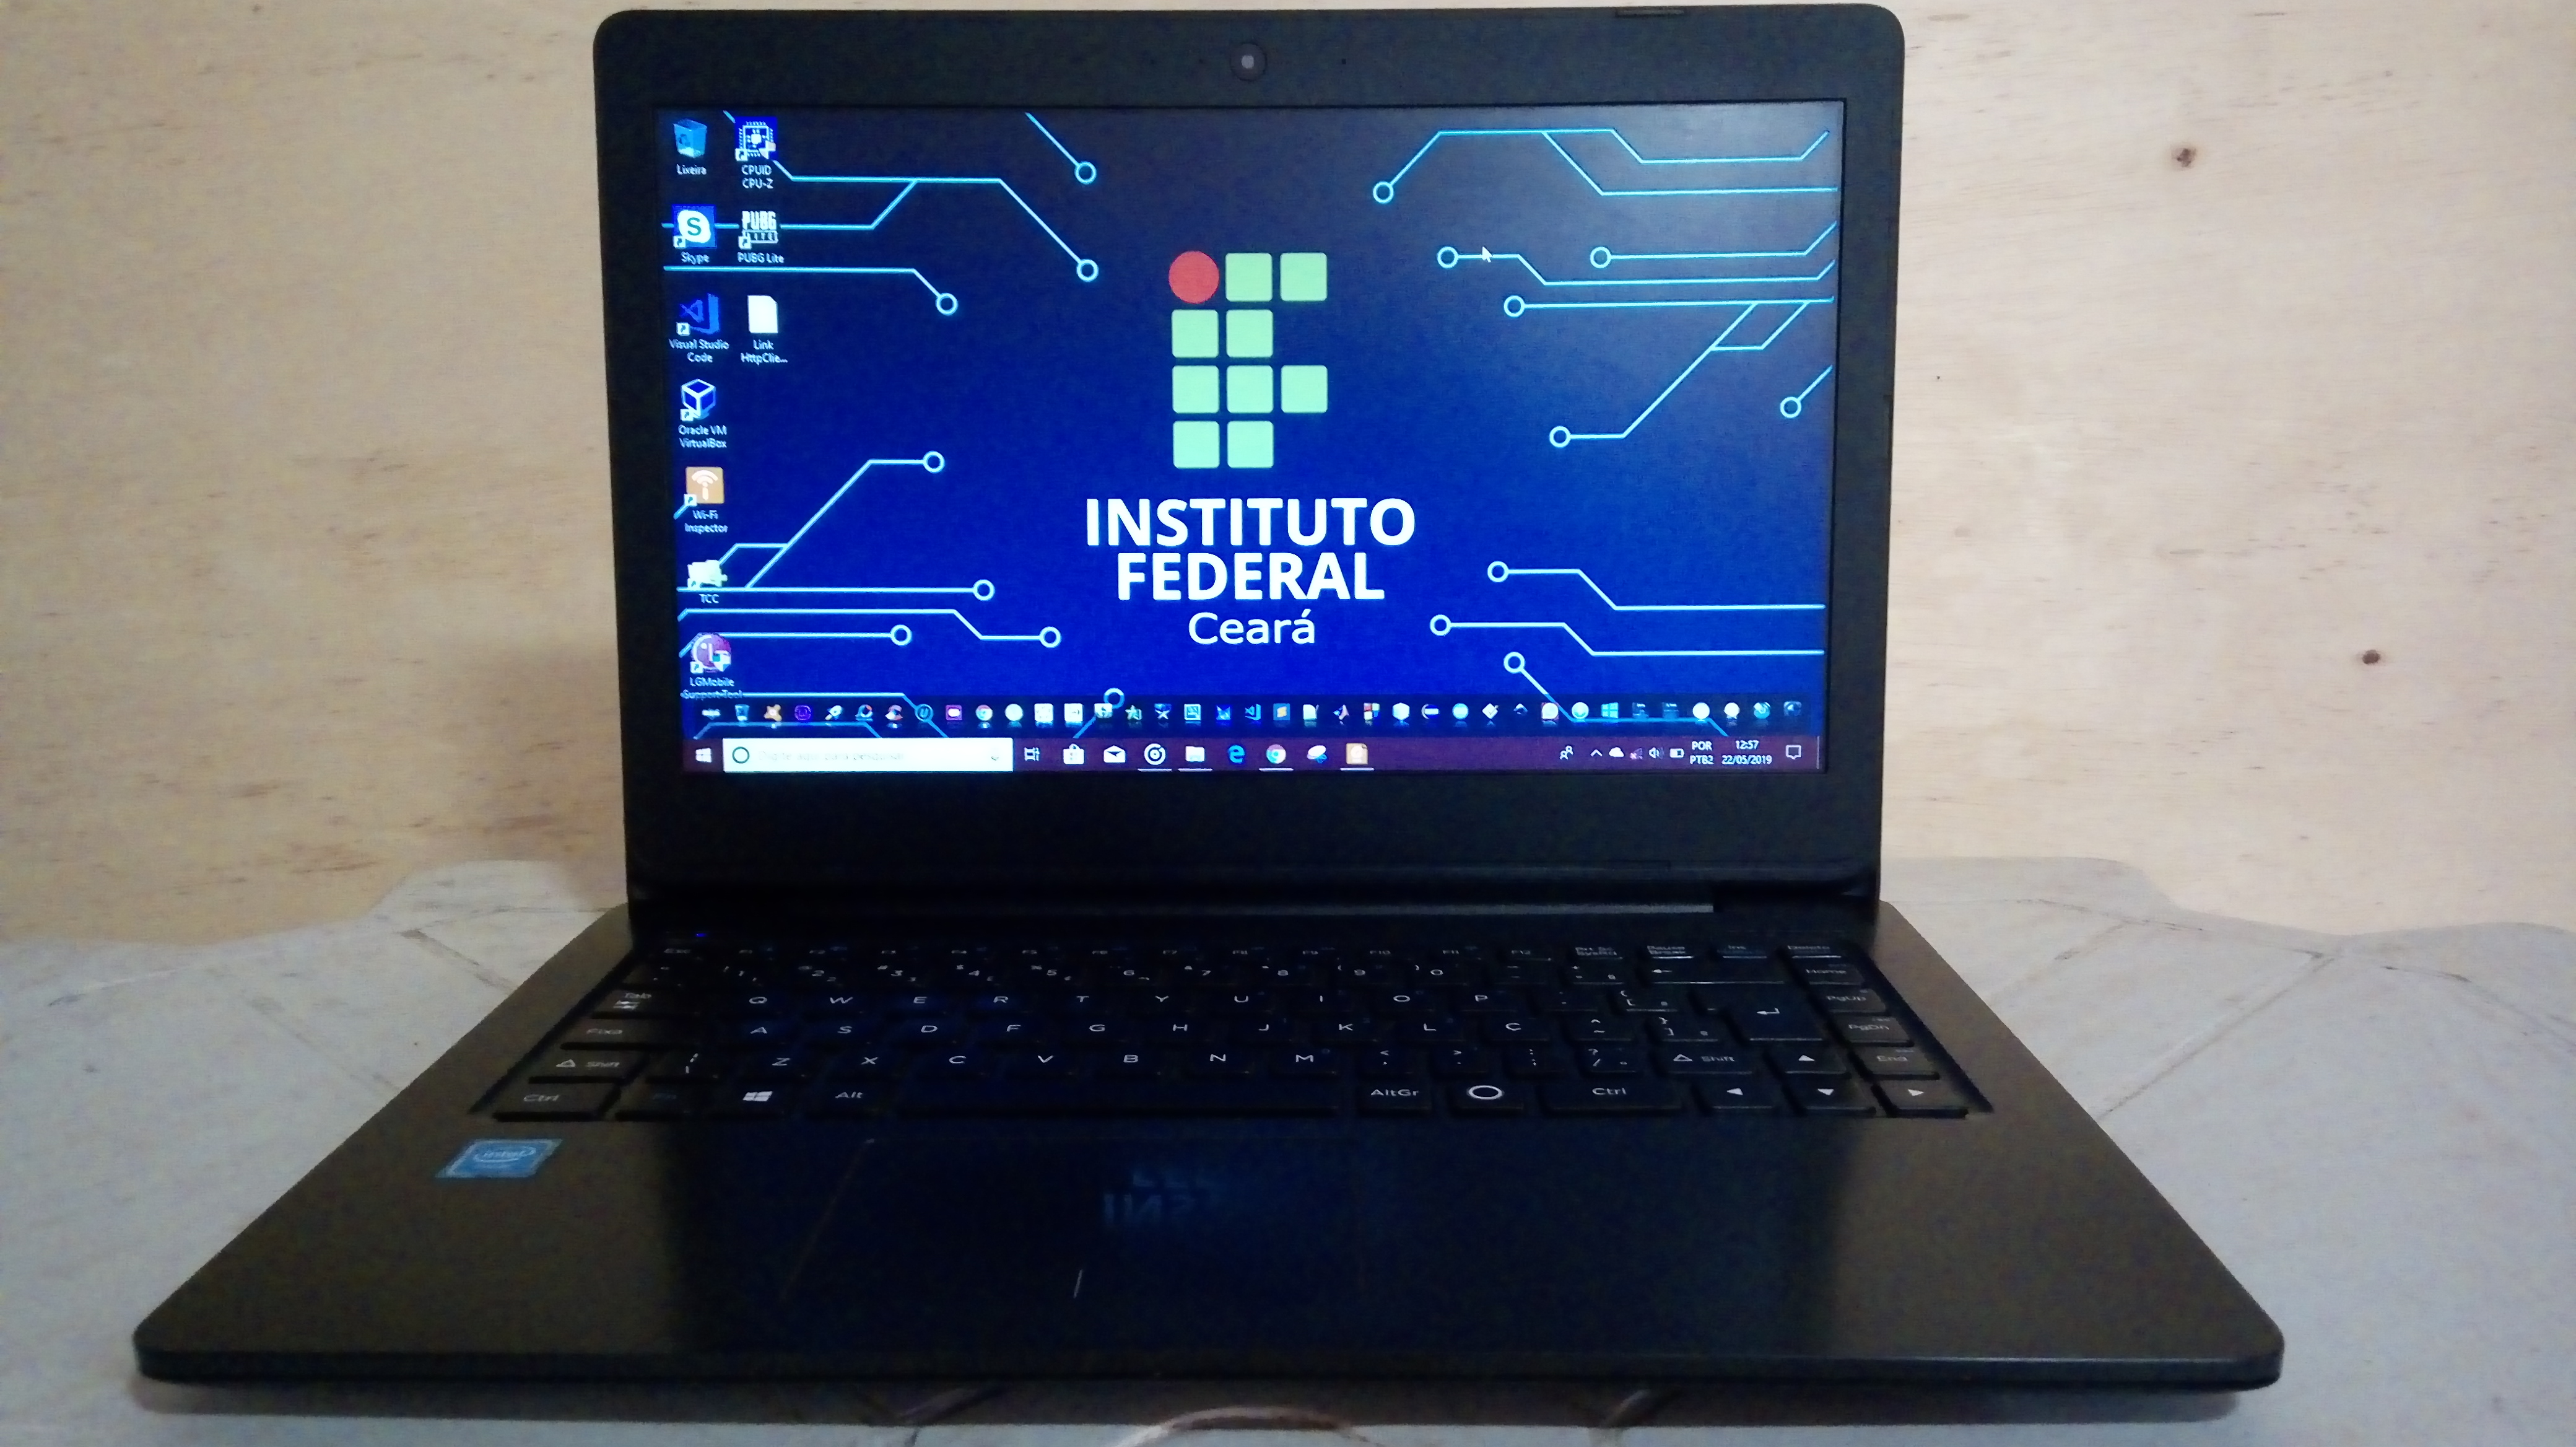
\includegraphics[scale=.1]{figuras/notebook.jpg}
	}{
		\Fonte{Autor.}%
	}	
\end{figure}

\begin{table}[H]
	\Caption{\label{tab:carac-notebook}Especificações do \textit{notebook} utilizado.}%
	\IBGEtab{}{%
		\begin{tabular}{ll}
			\toprule
			\multicolumn{1}{c}{Características do sistema} & \multicolumn{1}{c}{Descrição} \\
			\toprule %\midrule
			Modelo & Positivo S14BW01 \\
			
			Sistema Operacional & Windows 10 Pro 64 bits \\
			
			Memória RAM & 4 GB \\
			
			Processador & Intel Celeron N3060 @1.60GHz (2 CPUs) \\
			
			Placa de rede & Intel Dual Band Wireless-AC 3160 \\
			\bottomrule
		\end{tabular}%
	}{%
		\Fonte{Autor.}%
	}%
\end{table}

\section{Execução do site survey}
\label{sec:execucao-site-survey}

O processo de \textit{site survey} desenvolvido no IFCE \textit{campus} Tauá, caracterizado como do tipo \textit{indoor}, foi dividido, para uma melhor execução, em quatro etapas que vão desde o início da coleta dos dados em campo até os resultados obtidos, definidas como se segue:

\begin{compactenum}
	\item Reconhecimento do local;
	\item Coleta dos dados;
	\item Tratamento dos dados;
	\item Geração dos mapas de calor.
\end{compactenum}

\subsection{Reconhecimento do local}
\label{subsec:reconhecimento-do-local}

Nesta primeira etapa do \textit{site survey}, após a instalação dos programas no \textit{notebook}, já citados, foi feita uma vistoria em toda a área correspondente ao Bloco Didático do campus com a objetivo de verificar a sua infraestrutura física, identificar possíveis pontos para a medição e a presença ou não de fontes de interferências.

O ambiente analisado abrange uma área do tipo \textit{indoor} por conter salas, e também \textit{outdoor} devido ao espaço livre no prédio, como os que estão no primeiro andar. As \autoref{fig:andar1} e \ref{fig:andar2} mostram alguns dos pontos que foram verificados.

\begin{figure}[H]
	\centering
	\Caption{\label{fig:andar1}Alguns dos locais inspecionados no 1º andar do Bloco Didático.}	
	\UECEfig{}{
		\includegraphics[scale=.2]{figuras/Andar01.png}
	}{
		\Fonte{Autor.}%
	}	
\end{figure}

\begin{figure}[H]
	\centering
	\Caption{\label{fig:andar2}Alguns dos locais inspecionados no 2º andar do Bloco Didático.}	
	\UECEfig{}{
		\includegraphics[scale=.12]{figuras/Andar02.png}
	}{
		\Fonte{Autor.}%
	}	
\end{figure}

\subsection{Coleta dos dados}
\label{subsec:coleta-de-dados}

Nesta etapa foi iniciado o procedimento de medição dos níveis de potência, com a finalidade de obter informações das redes sem fio no \textit{campus} Tauá, sobretudo da cobertura das mesmas. O acesso e a utilização da planta baixa do Bloco Didático favoreceram para que fosse possível identificar a localização dos pontos de acesso e a estrutura física da instituição.

No Ekahau HeatMapper foi carregada a imagem da planta baixa do Bloco Didático. Logo após essa configuração, foi iniciado a demarcação dos pontos de medição por todo o local.

As primeiras medições ocorreram nos ambientes do tipo \textit{indoor} do Bloco Didático, o que inclui salas e laboratórios. Após a coleta dos níveis do sinal da rede de toda a parte interna, foi feita a captura na parte externa, como os corredores e locais sociais frequentados pelos estudantes. Em todo o prédio foram primeiramente analisados o segundo andar, e posteriormente o primeiro.

Para que todos os valores de medição obtidos na coleta fossem os mais precisos possível, foi feita uma comparação entre o ponto da planta baixa no Ekahau HeatMapper e o local da área real. Com isso, toda vez que um ponto de medida foi gerado, se obteve as potências de todas as redes Wi-Fi que estavam ao alcance do \textit{notebook}.

As medições ocorreram em 18 de maio de 2019 (sábado), pelo fato de que nesta data todos os docentes e discentes estariam ausentes do \textit{campus}. Isso contribuiu para que todas as salas e áreas que o Bloco Didático dispõe fossem visitadas e mapeadas.

A \autoref{fig:pontos-andar2} mostra os 62 pontos marcados no segundo andar do Bloco Didático, cada ponto vermelho na figura significa um local que foi medido a potência de sinal da rede Wi-Fi. Já a \autoref{fig:pontos-andar1} apresenta todos os 50 pontos que foram medidos no primeiro andar do mesmo prédio.

\begin{figure}[H]
	\centering
	\Caption{\label{fig:pontos-andar2}Pontos de medida no 2º andar do Bloco Didático.}	
	\UECEfig{}{
		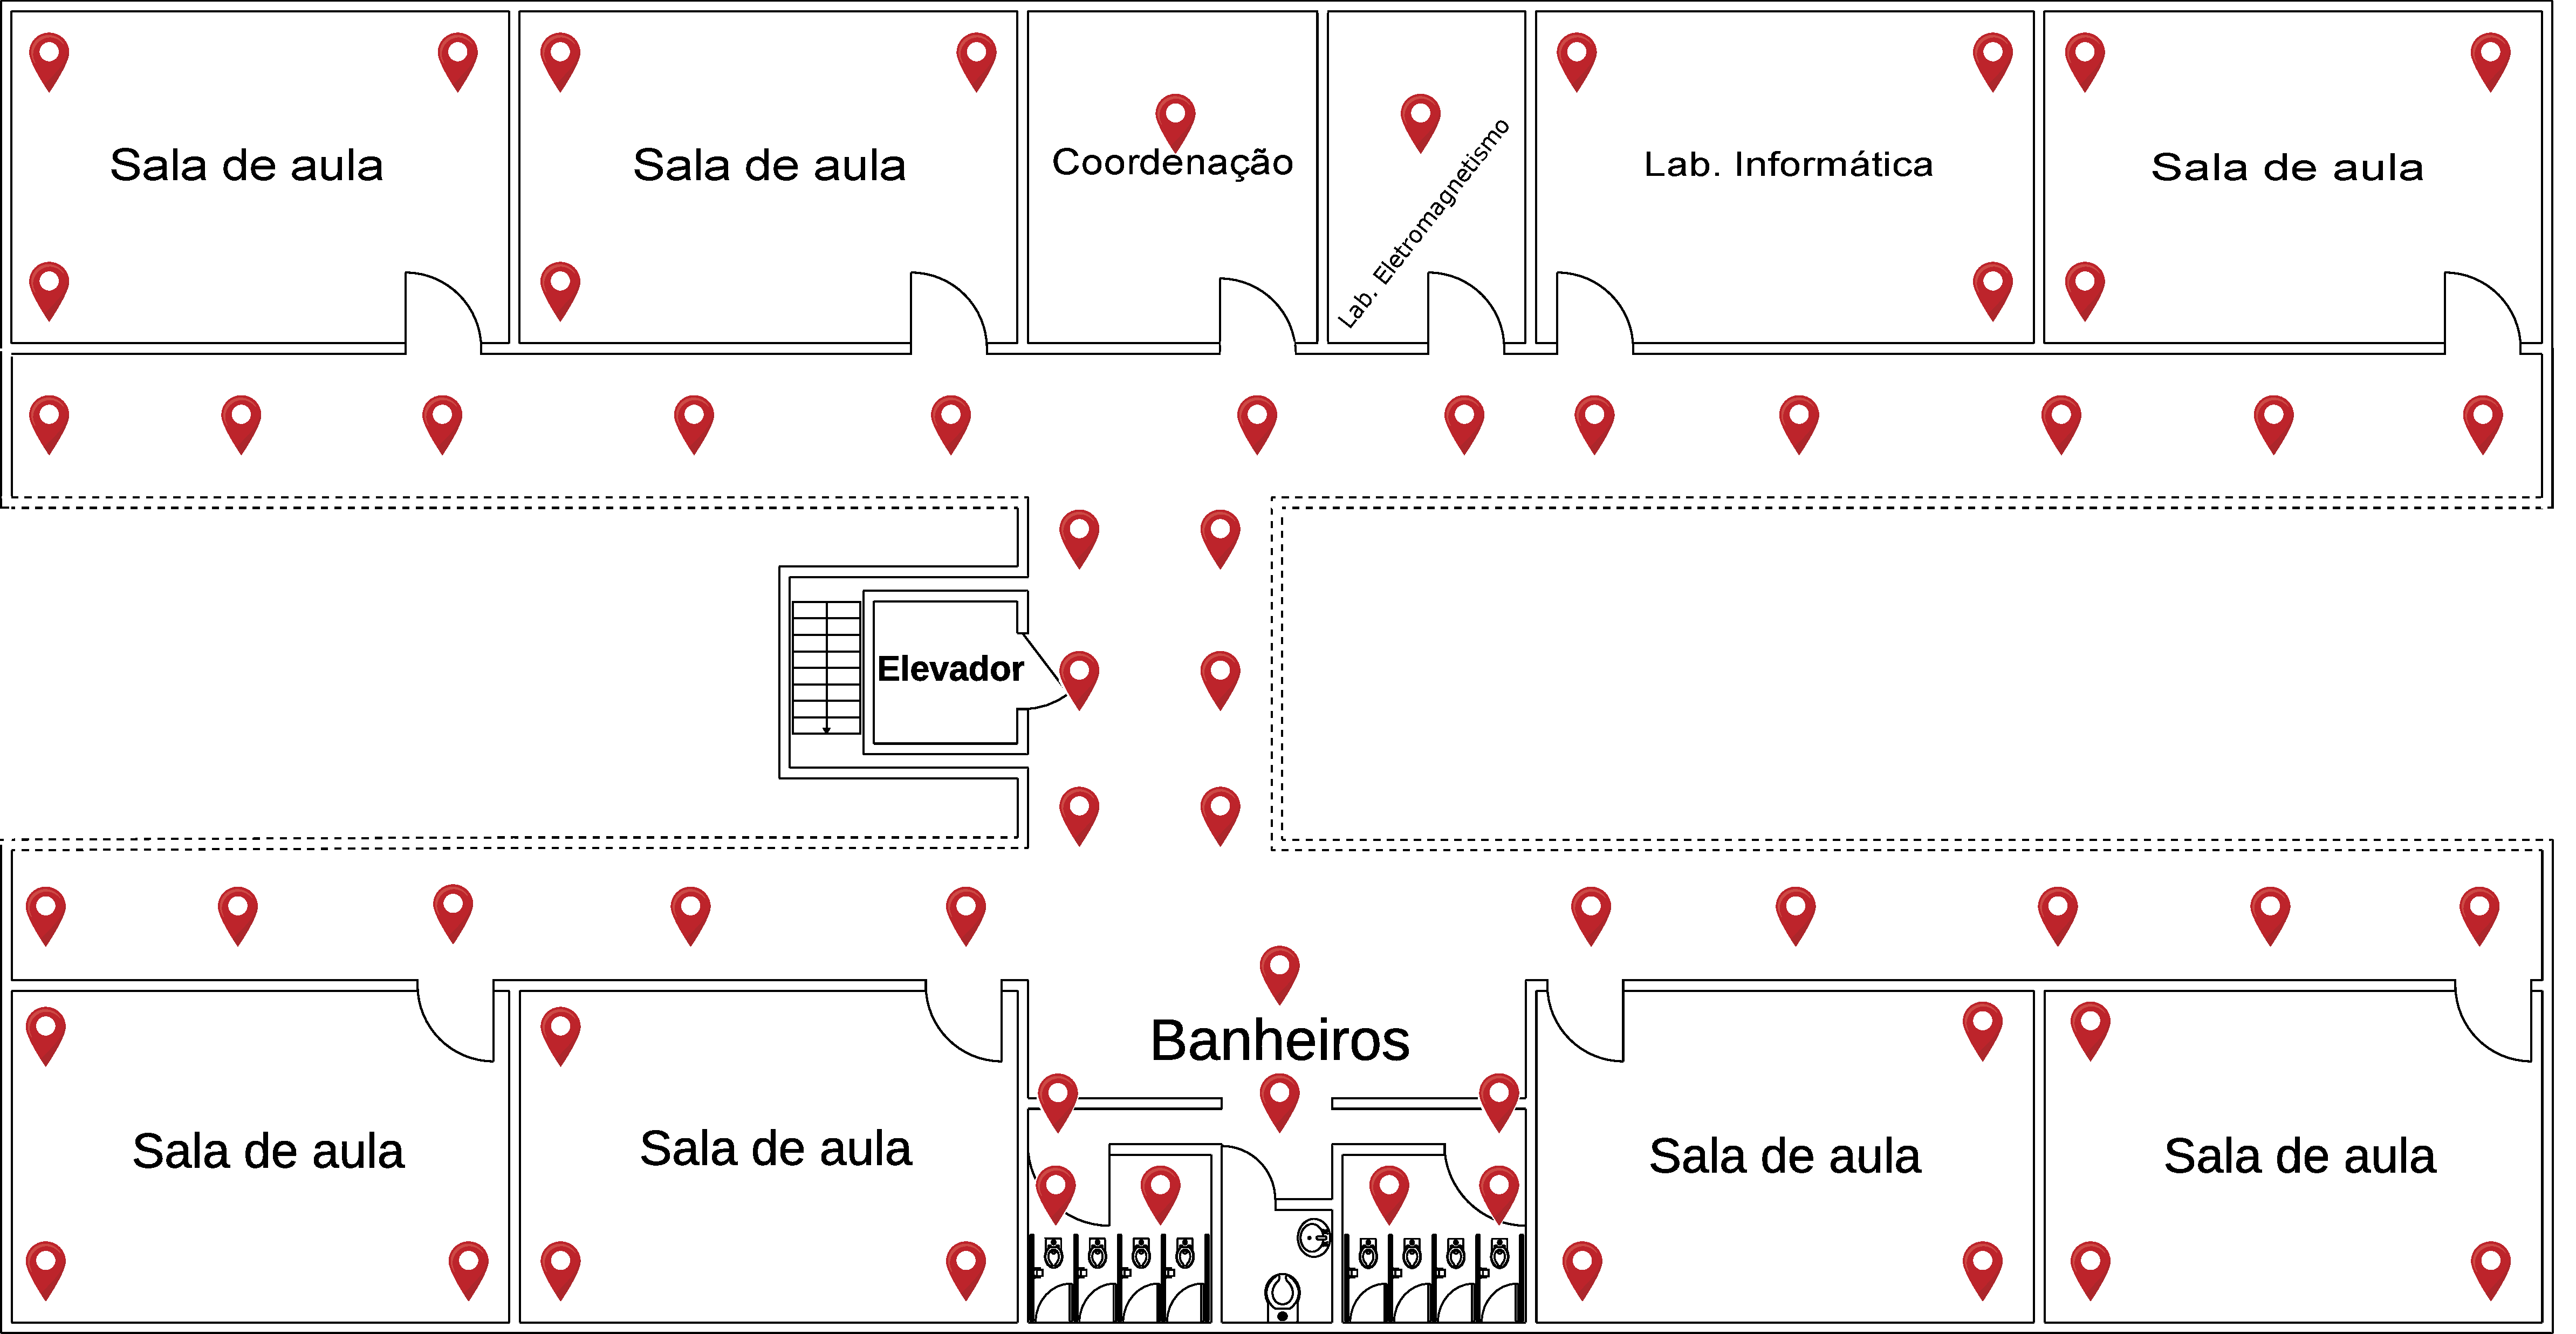
\includegraphics[scale=.24,angle=90]{figuras/Pontos_Medidos_Andar02.pdf}
	}{
		\Fonte{Autor.}%
	}	
\end{figure}

\begin{figure}[H]
	\centering
	\Caption{\label{fig:pontos-andar1}Pontos de medida no 1º andar do Bloco Didático.}	
	\UECEfig{}{
		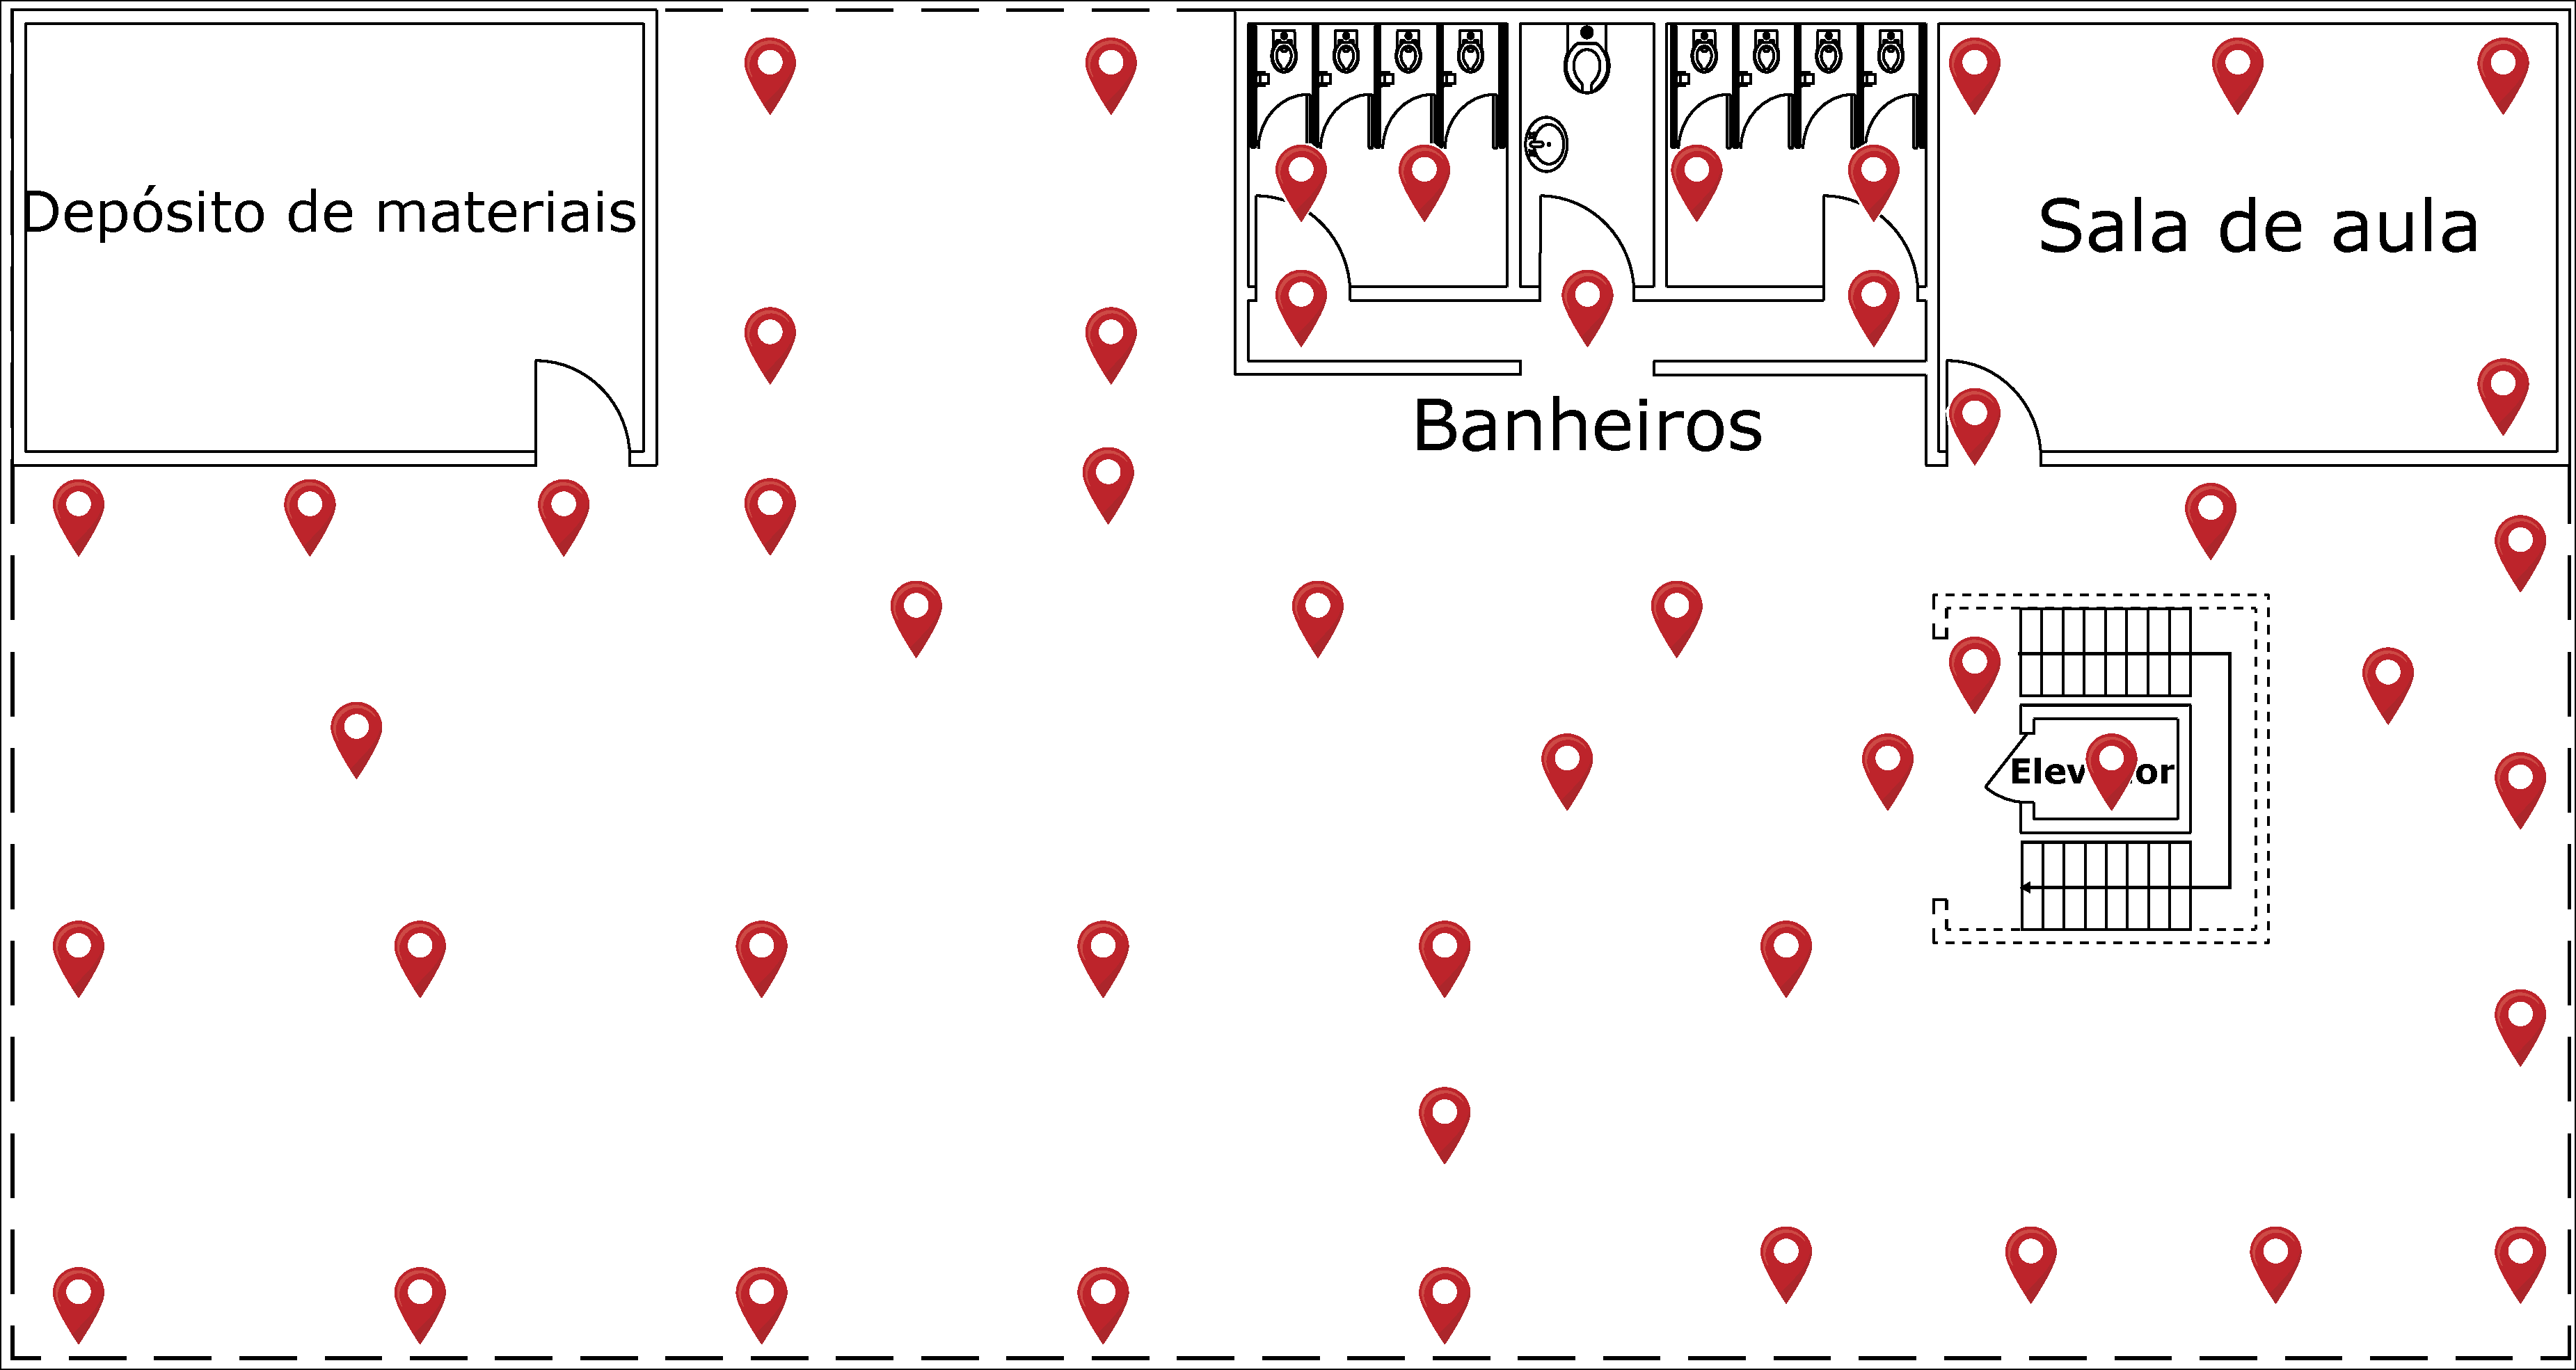
\includegraphics[scale=.37,angle=90]{figuras/Pontos_Medidos_Andar01.pdf}
	}{
		\Fonte{Autor.}%
	}	
\end{figure}

\subsection{Tratamento dos dados}
\label{subsec:tratamento-dos-dados}

Após a coleta dos dados das redes sem fio detectadas no Bloco Didático, iniciou-se a etapa de tratamento dos mesmos, no qual foram analisados e depois utilizados filtros para definir quais dados das redes capturadas seriam aproveitados.

A \autoref{fig:networks-didatico} mostra a lista criada no Xirrus Wi-Fi Inspector com as características dos pontos de acessos detectados na varredura no segundo andar do Bloco Didático. A princípio, ao ser gerada a lista, são exibidos o SSID e o nível do sinal das redes, e também são disponibilizadas informações como canal, protocolo de segurança, padrão 802.11 utilizado e o fabricante do equipamento.

\begin{figure}[H]
	\centering
	\Caption{\label{fig:networks-didatico}Redes Wi-Fi detectadas pelo Xirrus Wi-Fi Inspector.}	
	\UECEfig{}{
		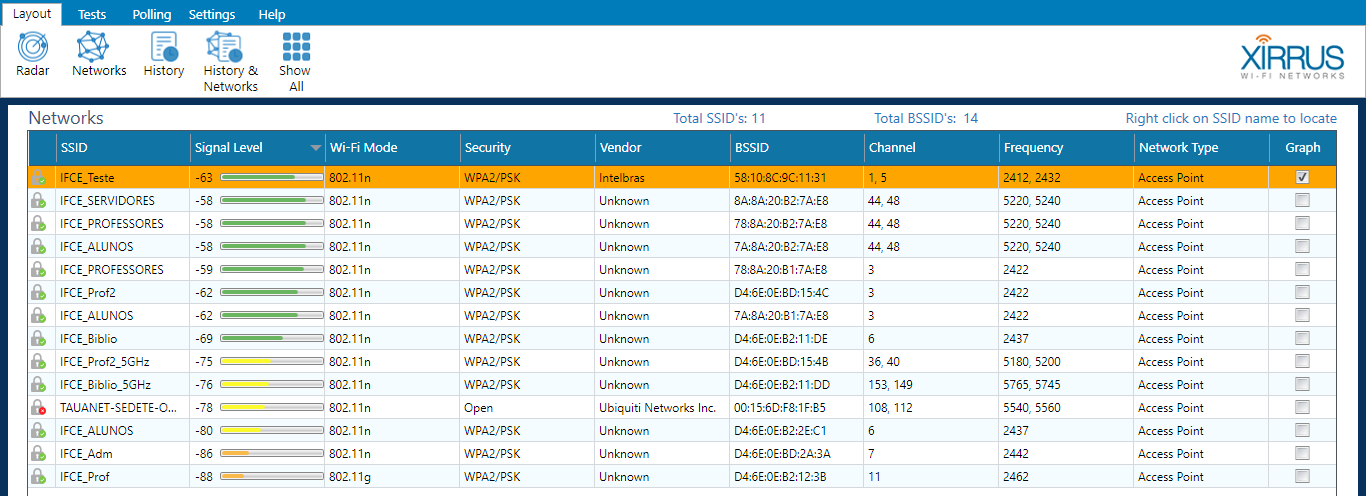
\includegraphics[scale=.43]{figuras/networks_didatic_recorte.png}
	}{
		\Fonte{Autor.}%
	}	
\end{figure}

\subsection{Geração dos mapas de calor}
\label{subsec:mapas-de-calor}

Depois de todas as etapas anteriores, no qual iniciou-se com o reconhecimento do local, e em seguida progrediu para a coleta das medidas de força do sinal e tratamento dos dados recolhidos, essa é última fase do \textit{site survey} que foi realizada, e consiste na exposição dos mapas de calor e os resultados alcançados durante o procedimento.

Um mapa de calor é uma representação gráfica de dados em que os valores são representados como cores com significados determinados. Em redes sem fio, podem ser utilizados para gerar um mapa da cobertura da intensidade do sinal em toda a área de interesse, o que favorece uma análise mais visual e simplificada do ambiente \textit{wireless}. Nesse sentido, são amplamente recomendados para a demonstração dos resultados obtidos em um \textit{site survey}.

Os mapas de calor no Ekahau HeatMapper são gerados a partir da coloração entre várias cores como verde, amarelo, laranja e vermelho, que são utilizadas para representarem as intensidades das potências recebidas em um determinado ponto.

A \autoref{fig:escala-sinal} demonstra a barra de potência do Ekahau HeatMapper que pode receber uma variação de cores desde do verde ao vermelho.

\begin{compactitem}
	\item \textbf{Verde:} significa que o sinal recebido é muito forte.
	\item \textbf{Amarelo:} significa que a potência recebida é razoável.
	\item \textbf{Laranja:} significa que a potência obtida ainda é aceitável.
	\item \textbf{Vermelho:} significa que a potência do sinal recebido é muito fraco.
\end{compactitem}

\begin{figure}[H]
	\centering
	\Caption{\label{fig:escala-sinal}Escala de potência do sinal.}	
	\UECEfig{}{
		
\includegraphics[scale=.185]{figuras/Escala_dBm.pdf}
	}{
		\Fonte{Autor.}%
	}	
\end{figure}

Para que os mapas fossem gerados foram definidos valores de potência baseados em testes de distância entre um ponto de acesso e o \textit{notebook}, no qual --85dBm (ou menor) representa uma área de sombra, isto é, sem propagação suficiente de sinal, e no mapa aparecerá a tonalidade mais forte de vermelho. Isso significa que toda área do mapa que receber esse nível de sinal será considerada de perda de conectividade. Caso a potência recebida no mapa for de --45dBm (ou maior, caso o receptor seja capaz de detectá-la), isto significa que o local mapeado possui alta conectividade, sendo assim representada pela cor verde.
